\documentclass[a4paper, amsfonts, amssymb, amsmath, reprint, showkeys, nofootinbib, twoside]{revtex4-1}
\usepackage[english]{babel}
\usepackage[utf8]{inputenc}
\usepackage[colorinlistoftodos, color=green!40, prependcaption]{todonotes}
\usepackage[pdftex, pdftitle={Article}, pdfauthor={Author}]{hyperref}
\usepackage{amsthm}
\usepackage{mathtools}
\usepackage{physics}
\usepackage{xcolor}
\usepackage{caption}
\usepackage{hyperref}
%\hypersetup{colorlinks=true, linkcolor=blue, urlcolor = blue}
\usepackage{amsmath}
\usepackage{amssymb}
\usepackage{graphicx}
\graphicspath{Images}
\usepackage[left=23mm,right=13mm,top=35mm,columnsep=15pt]{geometry} 
\usepackage{adjustbox}
\usepackage{placeins}
\usepackage[T1]{fontenc}
\usepackage{float}
%\usepackage{longtable}
\usepackage{csquotes}
\usepackage{refstyle}
\usepackage{lipsum}

\begin{document}

\title{Determination of Band Gap Using UV-Vis Spectroscopy}
\author{Swaroop Ramakant Avarsekar}
\email{swaroop.avarsekar@niser.ac.in}
\affiliation{School of Physical Sciences, National Institute of Science Education and Research, HBNI, Jatni -752050, India}
\date{\today}

	
\begin{abstract}
This experiment aims to determine the band gap of CdSe and polymer using ultraviolet-visible spectrometer, where CdSe is indirect band gap material and polymer with direct band gap. The tools from Beer Lambert's Law, and Tauc's method help us to determine the optical band gap of the materials. The band gap of CdSe is $(1.562\pm0.011)$ eV and polymer is $(1.565\pm0.020)$ eV with percentage error as 8.11\% for CdSe.
\end{abstract}
	
\keywords{Beer-Lambert's law, Phonon, Band gap, Tauc plot}
	
\maketitle

\section{Theory}
Band gap is the energy gap required by electron to break free from bound state, i.e transition from top of valence band to bottom of conduction band. In case of direct band gap materials, at the same electron momentum (k) the transition is allowed whereas in indirect band gap materials the conduction band and valence band lie in different  electron momentum, as shown in figures (\ref{1}) and (\ref{2}).

\begin{figure}[H]
	\centering
	\includegraphics[scale=0.3]{1}
	\caption{Direct band gap having same electron momentum}
	\label{1}
\end{figure}

\begin{figure}[H]
	\centering
	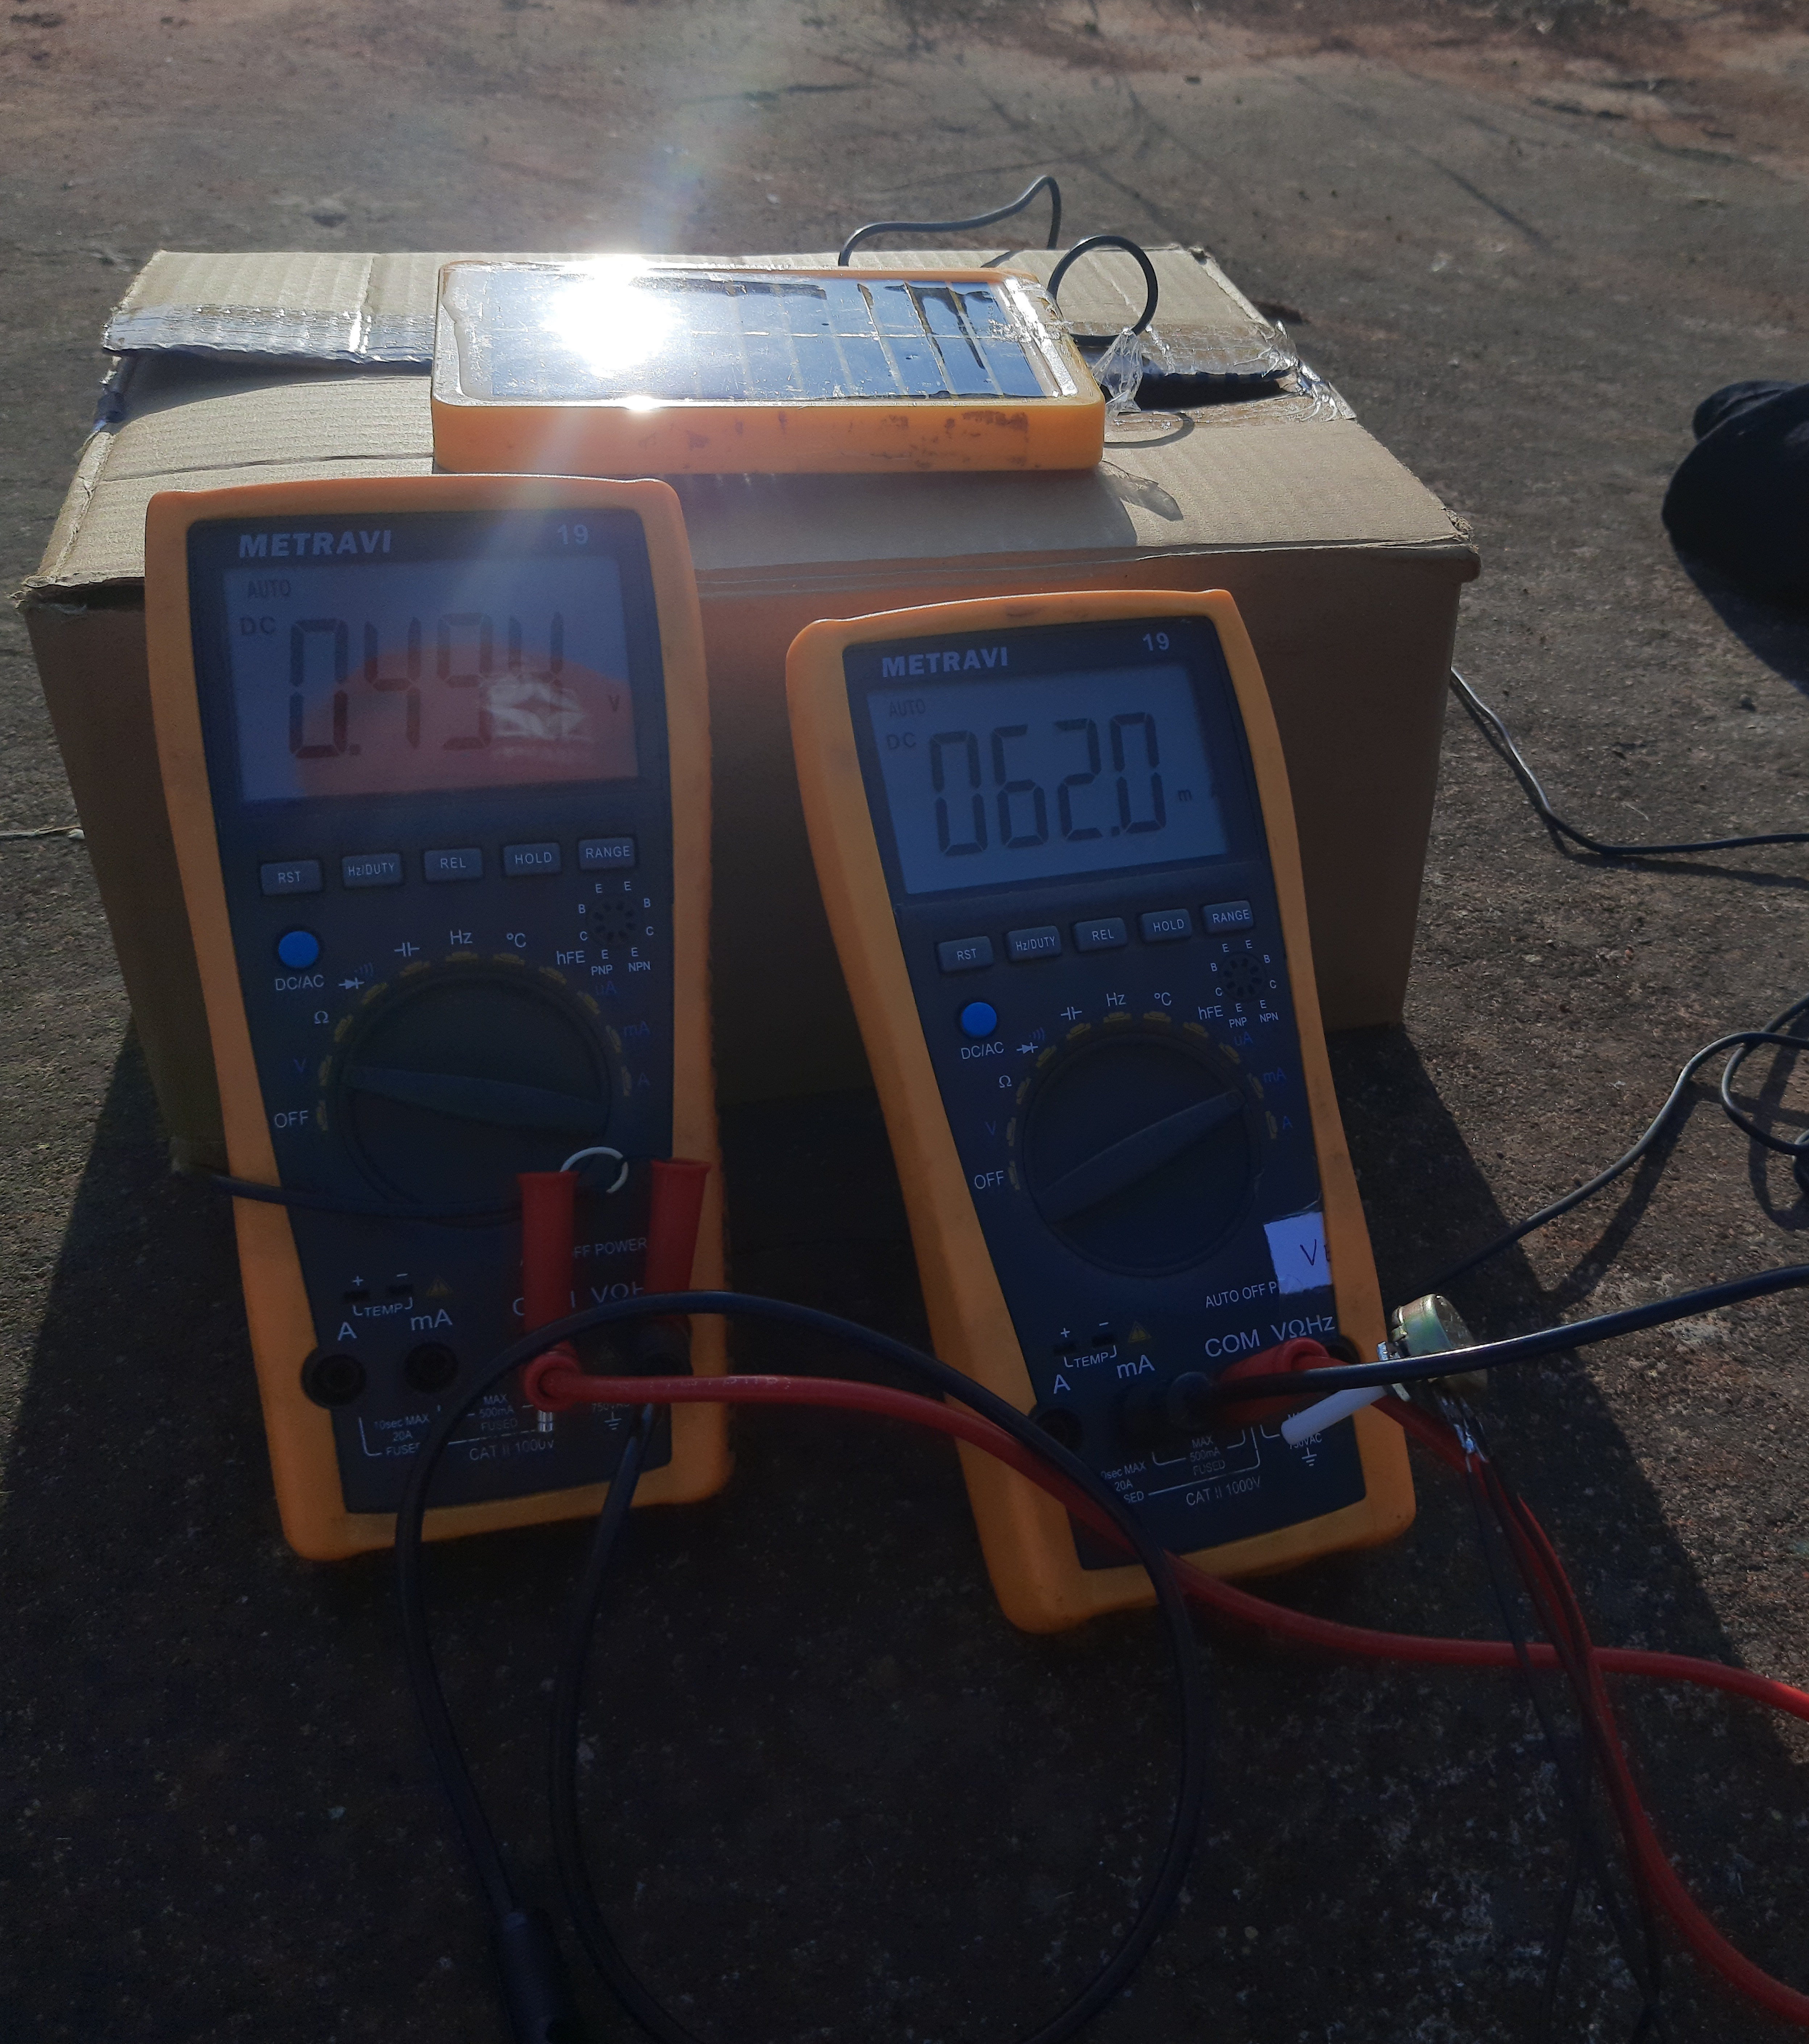
\includegraphics[scale=0.3]{2}
	\caption{Indirect band gap having different electron momentum}
	\label{2}
\end{figure}

When a photon of energy equal to band gap, is incident on the material electron hole pair is created. In case of indirect band gap materials, electron must undergo change in momentum with phonon assisted transition to reach the conduction band from valence band.. Phonon is a vibrational motion of lattice at uniform frequency as described in quantum mechanical picture. Phonons conserve the momentum for indirect transitions. In indirect process requires three entities photon, phonon and electron, hence proceeds at a slower rate unlike direct process.

The absorbance of light is directly proportional to path length and concentration as stated in Beer-Lambert's Law as shown below. UV-Vis Spectrometer is used to estimate band gap. The absorbance is given by-

\begin{equation}
	A=\epsilon c l = -log(I_T/I_o)
\end{equation}

where $\epsilon$ is molar absorptivity coefficient, c is the concentration absorbing species, l is the path length.

The absorption coefficient is given by:
\begin{equation}
	\alpha=A.ln(10)/l
\end{equation}

Tauc plot will be used to determine the optical band gap in semi conductors, with photon energy on abscissa and $\alpha$ on ordinate axis. Extrapolating curve to abscissa gives the band gap of the material. However there lies a complexity in equation which Tauc plot will be using for direct and indirect band gaps determination.

For direct band gap materials,
\begin{equation}
	\alpha=A(h\nu-E_g)^{0.5}
\end{equation}

The plot is between $\alpha^2$ and energy to determine band gap.

For indirect band gap materials, 
\begin{equation}
	\alpha=A(h\nu-E_g\mp E_p)^{2}
\end{equation}

where $E_g$ and $E_p$ are band gap and phonon energy. The - sign is for phonon absorption and + sign is for phonon emission. The plot is between $\sqrt{\alpha}$ and energy to determine band gap. 

\section{Analysis}
For the case of direct band gap a polymer was used which was already provided by the instructor since the optical range is beyond the UV-Visible spectrum. For this the data was collected from advanced research laboratory. We obtained the data for CdSe material from the laboratory. For CdSe material which has direct band gap, the spectra is shown in following figures (3) to (6). 

\begin{figure}[H]
	\centering
	\includegraphics[scale=0.3]{Sample}
	\caption{Raw data for Sample spectra}
	\label{3}
\end{figure}

\begin{figure}[H]
	\centering
	\includegraphics[scale=0.3]{Dark}
	\caption{Dark spectra}
	\label{4}
\end{figure}

\begin{figure}[H]
	\centering
	\includegraphics[scale=0.3]{Ref}
	\caption{Reference spectra}
	\label{5}
\end{figure}

\begin{figure}[H]
	\centering
	\includegraphics[scale=0.3]{Abs}
	\caption{Absorbance spectra}
	\label{6}
\end{figure}

The absorption coeffiecient $\alpha$ was calculated and plotted with the energy. For direct band gap estimation, $\alpha^2$ vs energy was plotted and $\alpha^{1/2}$ vs energy for indirect band gap. The linear region is identified, with best fit to get slope and intercept, hence the x intercept for band gap estimation.

\subsection{CdSe}
The plots from absorption coefficient is shown in Figure (\ref{7}) and Figure (\ref{8}) .
\begin{figure}[H]
	\centering
	\includegraphics[scale=0.6]{cse}
	\caption{Plot of $\alpha^2$ vs energy for CdSe}
	\label{7}
\end{figure}

\begin{figure}[H]
	\centering
	\includegraphics[scale=0.6]{csef}
	\caption{Linear region identified in plot of $\alpha^2$ vs energy for CdSe}
	\label{8}
\end{figure}

The best fit equation for the linear region is:
\begin{equation}
	y=10030561575.972 x  -15673858275.814
\end{equation}

Substituting y=0 gives x intercept as 1.562 eV as band gap energy for CdSe. The error estimation is given by:

\begin{equation}
	\delta E_g=E_g\left( \sqrt{\left(\frac{ \delta m}{m}\right)^2+\left(\frac{ \delta c}{c}\right)^2 }\right) 
\end{equation}

where m and c are slope and x-intercept respectively.

\begin{equation}
	\frac{\delta E_g}{1.562}= \sqrt{\left(\frac{4.4686\times10^7}{1.0030\times10^{10}}\right)^2+\left(\frac{8.5877\times10^{7}}{1.5673\times10^{10}}\right)^2 }
\end{equation}

$\delta E_g$ for CdSe is 0.011 eV. 

Therefore, band gap of CdSe is $(1.562\pm0.011)$ eV.

The literature value of band gap of CdSe is 1.70. The percentage error is 8.11\%.

\subsection{Polymer}
The plots from absorption coefficient is shown in Figure (\ref{9}) and Figure (\ref{10}) .
\begin{figure}[H]
	\centering
	\includegraphics[scale=0.6]{pol}
	\caption{Plot of $\alpha^{1/2}$ vs energy for Polymer}
	\label{9}
\end{figure}

\begin{figure}[H]
	\centering
	\includegraphics[scale=0.6]{polf}
	\caption{Linear region identified in plot of $\alpha^{1/2}$ vs energy for Polymer}
	\label{10}
\end{figure}

The best fit equation for the linear region is:
\begin{equation}
	y=0.539 x - 0.844
\end{equation}

Substituting y=0 gives x intercept as 1.565 eV as band gap energy for polymer. The error estimation is given by:

\begin{equation}
	\delta E_g=E_g\left( \sqrt{\left(\frac{ \delta m}{m}\right)^2+\left(\frac{ \delta c}{c}\right)^2 }\right) 
\end{equation}

where m and c are slope and x-intercept respectively.

\begin{equation}
	\frac{\delta E_g}{1.565}= \sqrt{\left(\frac{0.005}{0.539}\right)^2+\left(\frac{0.008}{0.844}\right)^2 }
\end{equation}

$\delta E_g$ for polymer is 0.020 eV. 

Therefore, band gap of polymer is $(1.565\pm0.020)$ eV. 

The exact material is not yet known but the band gap value may correspond to Polyacetylene based on table at reference (\ref{x}). The phonon energy was negligible and could not be distinguished in the plot, hence it was not considered in the calculations

\section{Conclusion}
This experiment was successful in estimation of band gap of CdSe and a polymer. The CdSe has direct bandgap whereas polymer had indirect. The optical range for CdSe was in UV-Visible range hence the UV-Visible spectrometer was used but for polymer, due to its optical range beyond UV-Visible range, the data was obtained from advanced research laboratory. With the parameters such as absorption coefficient and energy, we determine the band gap

We estimated the band gap energy for CdSe as $(1.562\pm0.011)$ eV and band gap of polymer is $(1.565\pm0.020)$ eV. The literature value of band gap of CdSe is 1.70. The percentage error was found to be 8.11\%. For polymer, the exact composition of material was not known but may closely correspond to Polyacetylene. We also had to approximate the energy of phonon for case of polymer since the transition could not be distinguished in the plot and had to be neglected.

Most of the data was collected digitally but few conditions may have contributed to the error. While measuring dark data spectrum, total darkness condition cannot be setup with the lid. Some of them may also include deposition/ contamination of the material used. However, care should be taken to maintain mechanically stable setup and storing material in safe place preventing contamination.

\section{References}
\begin{enumerate}
\item{\url{https://www.pveducation.org/pvcdrom/pn-junctions/band-gap}}
%\item {\url{}}
\item{\url{https://en.wikipedia.org/wiki/Direct_and_indirect_band_gaps}}
\item {\url{https://en.wikipedia.org/wiki/Phonon}}
\item{\url{https://www.niser.ac.in/sps/sites/default/files/basic_page/p347_2023/2.Bandgap_estimation_Uv-Vis_spectra.pdf}}
\item {\url{https://www.researchgate.net/figure/Energy-band-gap-and-conductivities-of-some-important-conducting-polymers-6_tbl1_325313568}}\label{x}

\end{enumerate}

\end{document}